\documentclass{beamer}
\usepackage[utf8]{inputenc}

\usetheme{Madrid}
\usecolortheme{default}
\usepackage{amsmath,amssymb,amsfonts,amsthm}
\usepackage{txfonts}
\usepackage{tkz-euclide}
\usepackage{listings}
\usepackage{adjustbox}
\usepackage{array}
\usepackage{tabularx}
\usepackage{gvv}
\usepackage{lmodern}
\usepackage{circuitikz}
\usepackage{tikz}
\usepackage{graphicx}

\setbeamertemplate{page number in head/foot}[totalframenumber]

\usepackage{tcolorbox}
\tcbuselibrary{minted,breakable,xparse,skins}



\definecolor{bg}{gray}{0.95}
\DeclareTCBListing{mintedbox}{O{}m!O{}}{%
  breakable=true,
  listing engine=minted,
  listing only,
  minted language=#2,
  minted style=default,
  minted options={%
    linenos,
    gobble=0,
    breaklines=true,
    breakafter=,,
    fontsize=\small,
    numbersep=8pt,
    #1},
  boxsep=0pt,
  left skip=0pt,
  right skip=0pt,
  left=25pt,
  right=0pt,
  top=3pt,
  bottom=3pt,
  arc=5pt,
  leftrule=0pt,
  rightrule=0pt,
  bottomrule=2pt,
  toprule=2pt,
  colback=bg,
  colframe=orange!70,
  enhanced,
  overlay={%
    \begin{tcbclipinterior}
    \fill[orange!20!white] (frame.south west) rectangle ([xshift=20pt]frame.north west);
    \end{tcbclipinterior}},
  #3,
}
\lstset{
    language=C,
    basicstyle=\ttfamily\small,
    keywordstyle=\color{blue},
    stringstyle=\color{orange},
    commentstyle=\color{green!60!black},
    numbers=left,
    numberstyle=\tiny\color{gray},
    breaklines=true,
    showstringspaces=false,
}
%------------------------------------------------------------
%This block of code defines the information to appear in the
%Title page
\title %optional
{1.4.19}
\date{August 26, 2025}
%\subtitle{A short story}

\author % (optional)
{Aditya Appana - EE25BTECH11004}



\begin{document}


\frame{\titlepage}
\begin{frame}{Question}
Find a point on the X axis, which is equidistant from the points 
\begin{align*}
\myvec{ 7 \\ 6 }\text{ and }\myvec{3 \\ 4}
\end{align*}

\end{frame}
\begin{frame}{allowframebreaks}
\frametitle{Given Information}

    \centering
    
    \label{tab:parameters}
    
    
    Let vector $\mathbf{P}$ be: \begin{align}
    \myvec{ 7\\6 }
    \end{align}
    

    Let vector $\mathbf{Q}$ be: \begin{align}\myvec{ 3\\4}\end{align}
    \label{0.2}

   
\end{frame}


\begin{frame}{Formula}
The formula to calculate the x-coordinate of the point $\vec{R}$ is

\vspace{1cm}

$$x= \frac{ ||\mathbf{P}||^2 - ||\mathbf{Q}||^2 }{2\mathbf{(P-Q)^T e_1}}$$

\end{frame}

\begin{frame}{allowframebreaks}
\frametitle{Solution}

    Substituting $\mathbf{P, Q}$, and $e_1$ in this formula :


$$x = \frac{7^2+6^2-(3^2+4^2)}{2 \myvec{4 \\ 2}^T \myvec{1\\0}}$$


$$=\frac{60}{8}$$
$$= 7.5$$ \\

Therefore, the required point is (7.5,0)
\end{frame}




\begin{frame}[fragile]
    \frametitle{Python Code}
    \begin{lstlisting}
import sys 

import numpy as np
import matplotlib.pyplot as plt


def line_gen(A,B):
  len =10
  dim = A.shape[0]
  x_AB = np.zeros((dim,len))
  lam_1 = np.linspace(0,1,len)
  for i in range(len):
    temp1 = A + lam_1[i]*(B-A)
    x_AB[:,i]= temp1.T
  return x_AB
\end{lstlisting}
\end{frame}

\begin{frame}[fragile]
    \frametitle{Python Code}

    \begin{lstlisting}
v1 = np.array([7,6]).reshape(-1,1)
v2 = np.array([3,4]).reshape(-1,1)

e1 = np.array([1,0]).reshape(-1,1)

diff = (v1-v2).T

dot_product = diff@e1

denominator = 2*(dot_product)

norm1 = np.linalg.norm(v1)
norm1 = norm1*norm1

norm2 = np.linalg.norm(v2)
norm2 = norm2*norm2


    \end{lstlisting}
\end{frame}

\begin{frame}[fragile]
    \frametitle{Python Code}

    \begin{lstlisting}
R = (ratio*Q + P) / (ratio + 1)
#Calculating vector R with the first formula

S = (ratio*Q - P) / (ratio - 1)
#Calculating vector S with the second formula

    \end{lstlisting}
\end{frame}

\begin{frame}[fragile]
    \frametitle{Python Code}

    \begin{lstlisting}
xcoord = (norm1-norm2)/(denominator)
print(xcoord)

x = xcoord[0,0]


reqdpoint = np.array([x,0]).reshape(-1,1)



allcoords = np.block([v1,v2,reqdpoint])




x_1r = line_gen(v1,reqdpoint)
x_2r = line_gen(v2,reqdpoint)


\end{lstlisting}
\end{frame}

\begin{frame}[fragile]
    \frametitle{Python Code}

    \begin{lstlisting}

#Plotting all lines
plt.plot(x_1r[0,:],x_1r[1,:],label='$AB$')
plt.plot(x_2r[0,:],x_2r[1,:],label='$BC$')

#Labeling the coordinates
colors = np.arange(1,4)
allcoords = np.block([[v1,v2,reqdpoint]])
plt.scatter(allcoords[0,:], allcoords[1,:], c=colors)
vert_labels = ['v1','v2','required point']
for i, txt in enumerate(vert_labels):
    
    plt.annotate(f'{txt}\n({allcoords[0,i]:.2f}, {allcoords[1,i]:.2f})',
                 (allcoords[0,i], allcoords[1,i]), textcoords="offset points", xytext=(25,5), ha='center') 
\end{lstlisting}
\end{frame}

\begin{frame}[fragile]
    \frametitle{Python Code}

    \begin{lstlisting}
ax = plt.gca()
ax.spines['top'].set_color('none')
ax.spines['left'].set_position('zero')
ax.spines['right'].set_color('none')
ax.spines['bottom'].set_position('zero')

plt.grid() # minor
plt.axis('equal')

plt.show()
    \end{lstlisting}
\end{frame}


\begin{frame}{Plot}
\begin{figure}
    \centering
    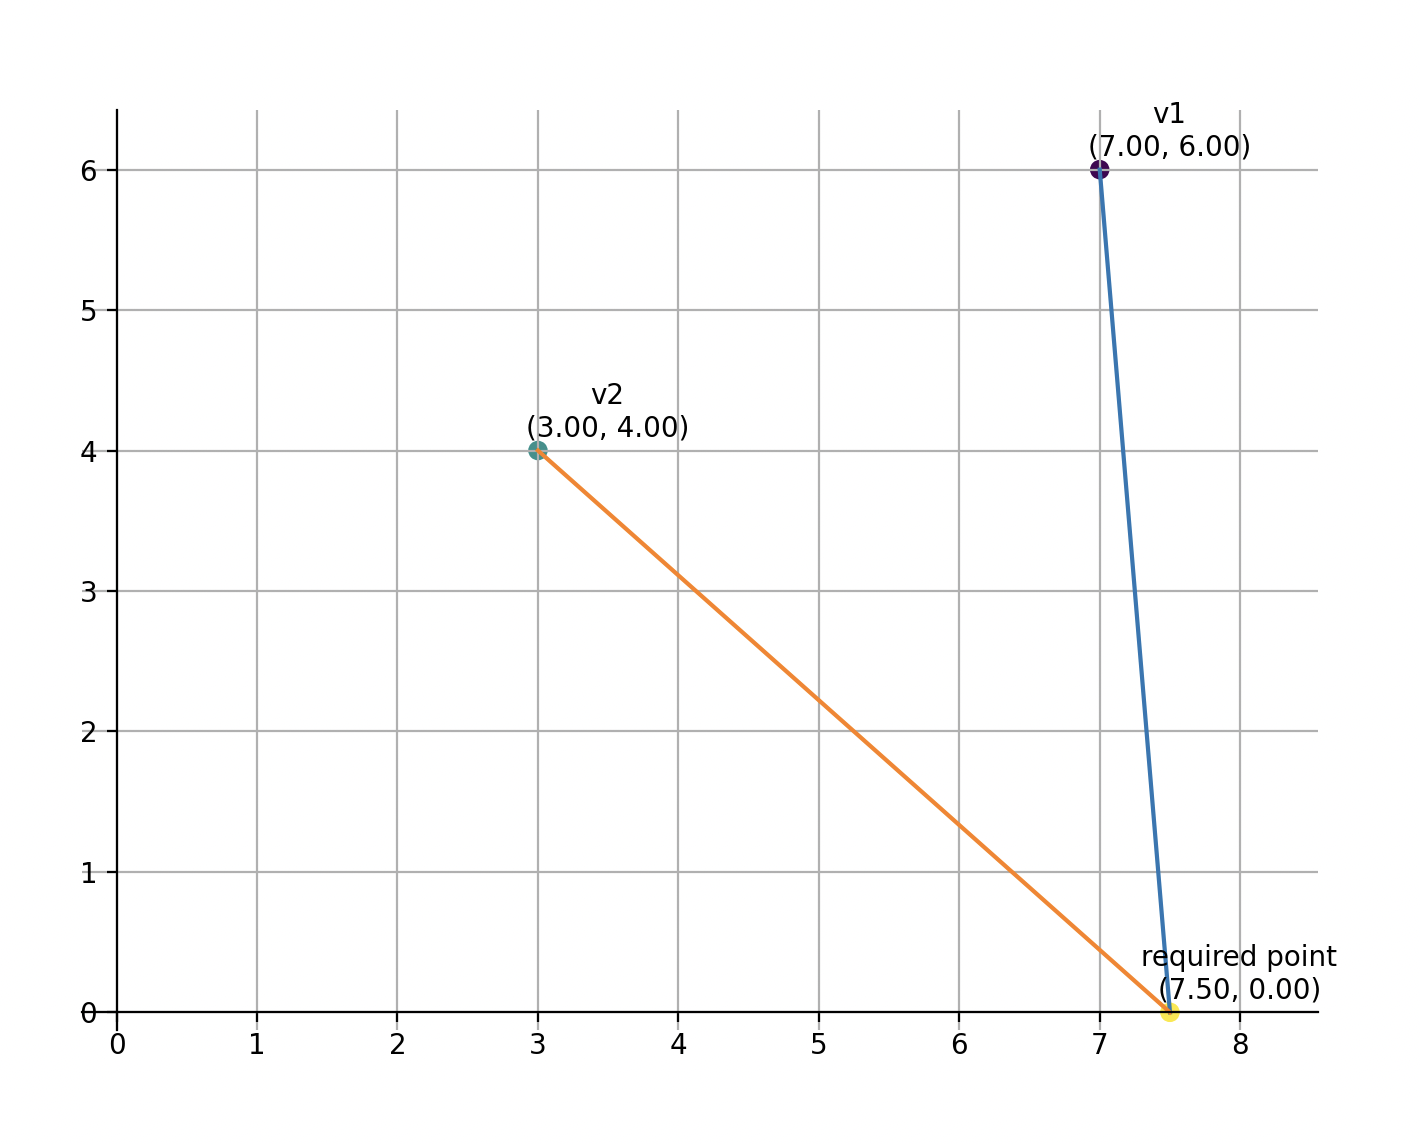
\includegraphics[width=0.8\columnwidth]{Figs/Figure_2.png}
    \caption{Plot}
    \label{fig:placeholder}
\end{figure}
\end{frame}

\begin{frame}[fragile]
\frametitle{C Code}
\begin{lstlisting}
#include<stdio.h>

float xfinder (float x1, float y1, float x2, float y2){

float norm1 = x1*x1 + y1*y1;

float norm2 = x2*x2 + y2*y2;

float denominator = x1 - x2;

float xcoord = (norm1 - norm2)/(2 * denominator);

return xcoord;
}




\end{lstlisting}

\end{frame}


\begin{frame}[fragile]
\frametitle{Python and C Code}

\begin{lstlisting}
import sys 
import ctypes

import numpy as np
import matplotlib.pyplot as plt


def line_gen(A,B):
  len =10
  dim = A.shape[0]
  x_AB = np.zeros((dim,len))
  lam_1 = np.linspace(0,1,len)
  for i in range(len):
    temp1 = A + lam_1[i]*(B-A)
    x_AB[:,i]= temp1.T
  return x_AB

\end{lstlisting}

\end{frame}

\begin{frame}[fragile]
\frametitle{Python and C Code}

\begin{lstlisting}
c_lib=ctypes.CDLL('./main.so')

# Define the argument types for the x function
c_lib.xfinder.argtypes = [ctypes.c_float, ctypes.c_float,ctypes.c_float, ctypes.c_float]
# Define the return type of the x function
c_lib.xfinder.restype = ctypes.c_float
# --- Define Points and Calculate 'm' using C function ---

v1 = np.array([7,6])
v2 = np.array([3,4])

xcoord = c_lib.xfinder(
    ctypes.c_float(v1[0]),
    ctypes.c_float(v1[1]), 
    ctypes.c_float(v2[0]), 
    ctypes.c_float(v2[1])
)
\end{lstlisting}

\end{frame}

\begin{frame}[fragile]
\frametitle{Python and C Code}
\begin{lstlisting}
v1 = np.array([7,6]).reshape(-1,1)
v2 = np.array([3,4]).reshape(-1,1)

reqdpoint = np.array([xcoord, 0]).reshape(-1,1)

allcoords = np.block([v1,v2,reqdpoint])




x_1r = line_gen(v1,reqdpoint)
x_2r = line_gen(v2,reqdpoint)

\end{lstlisting}
\end{frame}

\begin{frame}[fragile]
\frametitle{Python and C Code}
\begin{lstlisting}

#Plotting all lines
plt.plot(x_1r[0,:],x_1r[1,:],label='$AB$')
plt.plot(x_2r[0,:],x_2r[1,:],label='$BC$')

#Labeling the coordinates
colors = np.arange(1,4)
allcoords = np.block([[v1,v2,reqdpoint]])
plt.scatter(allcoords[0,:], allcoords[1,:], c=colors)
vert_labels = ['v1','v2','required point']
for i, txt in enumerate(vert_labels):
    #plt.annotate(txt, # this is the text
    plt.annotate(f'{txt}\n({allcoords[0,i]:.2f}, {allcoords[1,i]:.2f})',
                 (allcoords[0,i], allcoords[1,i]), textcoords="offset points", xytext=(25,5), ha='center') 
\end{lstlisting}
\end{frame}

\begin{frame}[fragile]
\frametitle{Python and C Code}
\begin{lstlisting}

# use set_position
ax = plt.gca()
ax.spines['top'].set_color('none')
ax.spines['left'].set_position('zero')
ax.spines['right'].set_color('none')
ax.spines['bottom'].set_position('zero')

plt.grid() # minor
plt.axis('equal')

plt.show()

\end{lstlisting}
\end{frame}

\begin{frame}{Plot}
\begin{figure}
    \centering
    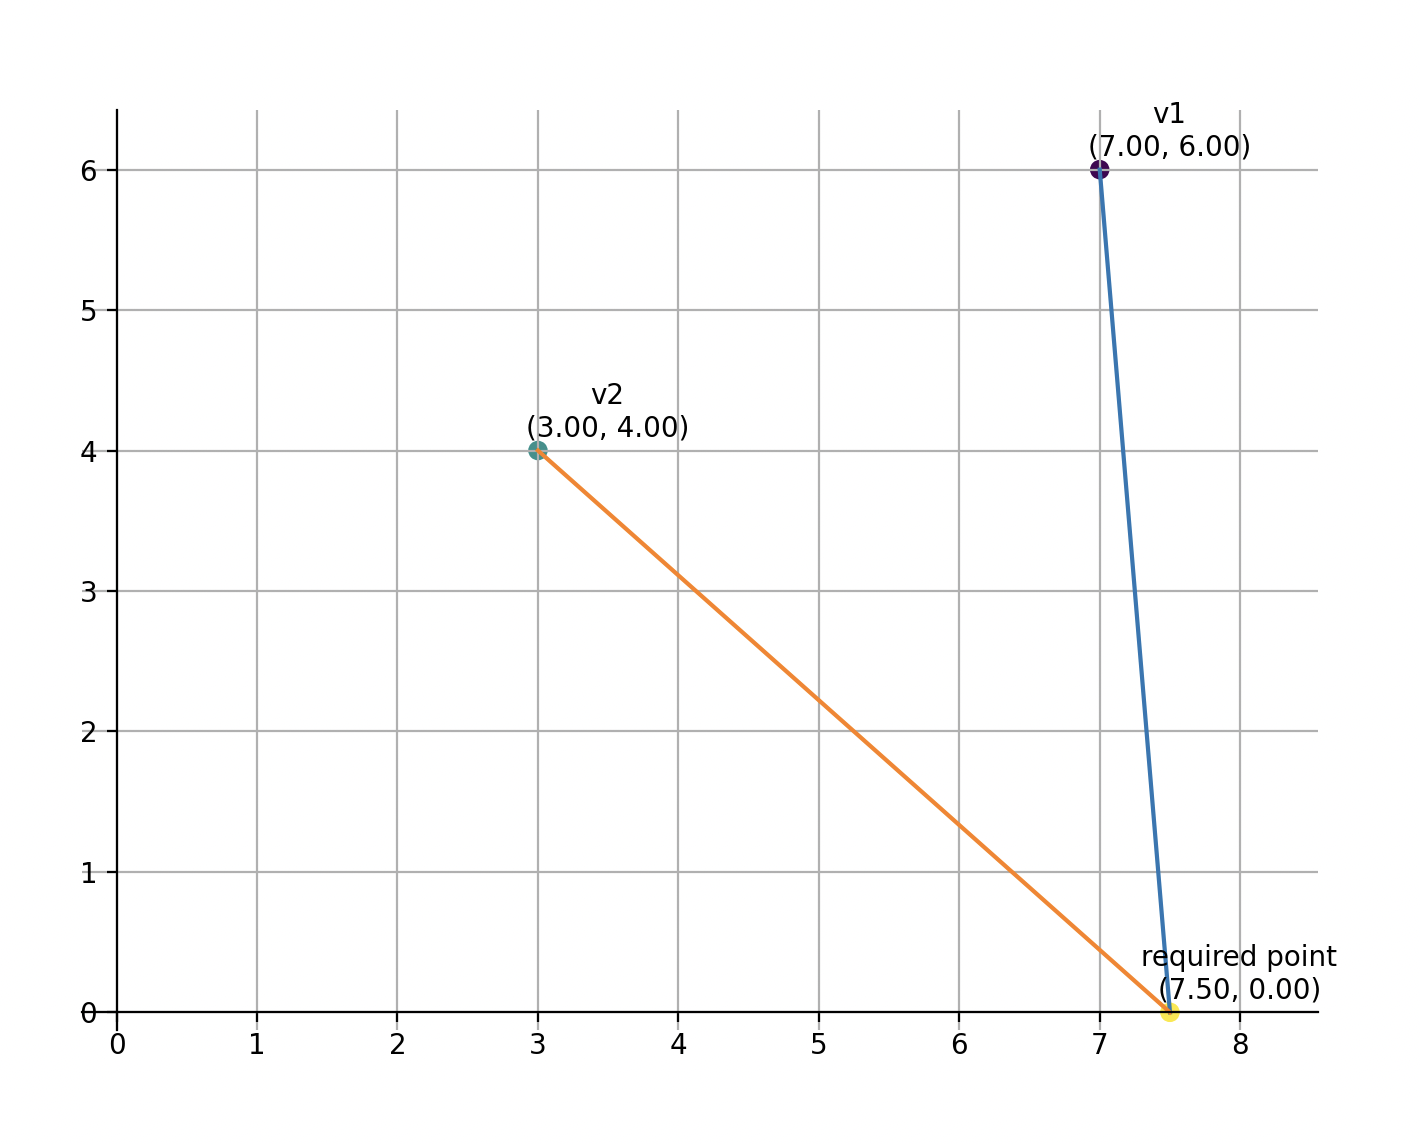
\includegraphics[width=0.8\columnwidth]{Figs/Figure_2.png}
    \caption{Plot}
    \label{fig:placeholder}
\end{figure}
\end{frame}

\end{document}